	\begin{center}
	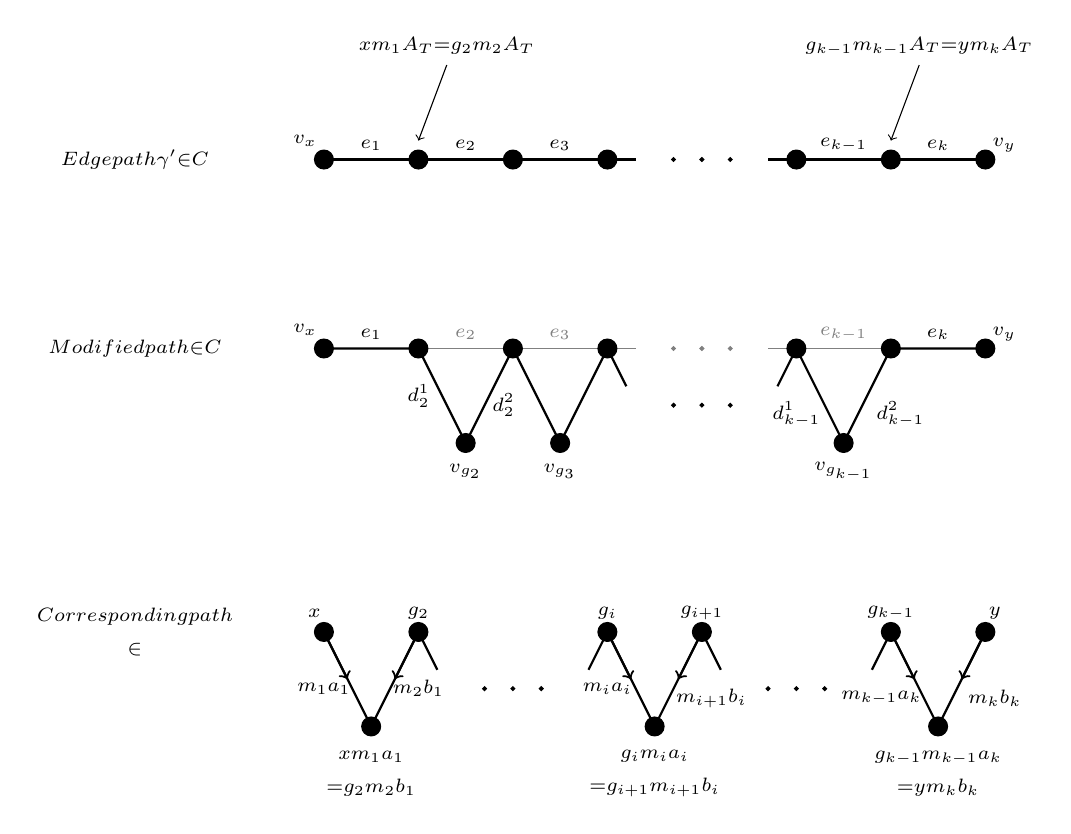
\begin{tikzpicture}[scale=1.2]
		\foreach \x in {0,1,2,3,5,6,7}
		\draw[fill=black] (\x,0) circle [radius=0.1];
		\draw[thick] (0,0) -- (3.3,0) (4.7,0)--(7,0);
		\foreach \x in {3.7,4,4.3}
		\draw[fill=black] (\x, 0) circle [radius=0.02];
		
		\draw[->] (1.3,1) --(1,0.2);
		\draw (1.3,1.2) node {$\scriptstyle{xm_1A_T=g_2m_2A_T}$};
		\draw[->] (6.3,1) --(6,0.2);
		\draw (6.3,1.2) node {$\scriptstyle{g_{k-1}m_{k-1}A_T=ym_kA_T}$};
		
				
		%labels
		\draw (-2,0) node {$\scriptstyle{\text{Edge path }\gamma' \in C\DG}$};
		\draw (-0.2,0.2) node{$\scriptstyle{v_x}$} (7.2,0.15) node{$\scriptstyle{v_y}$}(0.5,0.15) node{$\scriptstyle{e_1}$}(1.5,0.15) node{$\scriptstyle{e_2}$} (2.5,0.15) node{$\scriptstyle{e_3}$}(5.5,0.15) node{$\scriptstyle{e_{k-1}}$}(6.5,0.15) node{$\scriptstyle{e_k}$};

%modified path
	\draw[thin,gray] (0,-2) -- (3.3,-2) (4.7,-2)--(7,-2);
		\foreach \x in {0,1,2,3,5,6,7}
	\draw[fill=black] (\x,-2) circle [radius=0.1];
	\foreach \x in {3.7,4,4.3}
	\draw[gray, fill=gray] (\x, -2) circle [radius=0.02];
	
	\foreach \x in {1.5,2.5,5.5}
	\draw[fill=black] (\x,-3) circle [radius=0.1];
	\draw[thick] (0,-2) -- (1,-2) --(1.5,-3)--(2,-2)--(2.5,-3)--(3,-2)--(3.2,-2.4) (4.8,-2.4)--(5,-2)--(5.5,-3)--(6,-2)--(7,-2);
	\foreach \x in {3.7,4,4.3}
	\draw[fill=black] (\x, -2.6) circle [radius=0.02];
	
	%labels
	\draw (-2,-2) node {$\scriptstyle{\text{Modified path } \in C\DG}$};
	\draw (-0.2,-1.8) node{$\scriptstyle{v_x}$} (7.2,-1.85) node{$\scriptstyle{v_y}$}(0.5,-1.85) node{$\scriptstyle{e_1}$}(1.5,-1.85) node[gray]{$\scriptstyle{e_2}$} (2.5,-1.85) node[gray]{$\scriptstyle{e_3}$}(5.5,-1.85) node[gray]{$\scriptstyle{e_{k-1}}$}(6.5,-1.85) node{$\scriptstyle{e_k}$};
	
	\draw (1.5,-3.3) node{$\scriptstyle{v_{g_2}}$} (2.5,-3.3) node{$\scriptstyle{v_{g_3}}$} (5.5,-3.3) node{$\scriptstyle{v_{g_{k-1}}}$} (1,-2.5) node{$\scriptstyle{d^1_2}$} (1.9,-2.6) node{$\scriptstyle{d^2_2}$} (5,-2.7) node{$\scriptstyle{d^1_{k-1}}$} (6.1,-2.7) node{$\scriptstyle{d^2_{k-1}}$};
	
	
	%path in Cayley graph
	\foreach \x in {0,1,3,4,6,7}
	\draw[fill=black] (\x,-5) circle [radius=0.1];
	
	\foreach \x in {0.5,3.5,6.5}
	\draw[fill=black] (\x,-6) circle [radius=0.1];
	\draw[thick] (0,-5)-- (0.5,-6)-- (1,-5) --(1.2,-5.4)(2.8,-5.4)--(3,-5)--(3.5,-6)--(4,-5)--(4.2,-5.4) (5.8,-5.4)--(6,-5)--(6.5,-6)--(7,-5);
	\foreach \x in {1.7,2,2.3,4.7,5,5.3}
	\draw[fill=black] (\x, -5.6) circle [radius=0.02];
	\draw[thick, ->] (0,-5)--(0.25,-5.5) ;
	\draw[thick, ->](1,-5)--(0.75,-5.5) ;
	\draw[thick, ->] (3,-5)--(3.25,-5.5) ;
	\draw[thick, ->](4,-5)--(3.75,-5.5) ;
	\draw[thick, ->] (6,-5)--(6.25,-5.5) ;
	\draw[thick, ->](7,-5)--(6.75,-5.5) ;
	
	%labels
	\draw (-2,-5) node[align=center] {$\scriptstyle{\text{Corresponding path }}$\\$\scriptstyle{ \in \MCay}$};
	\draw (-0.1,-4.8) node{$\scriptstyle{x}$} (7.1,-4.8) node{$\scriptstyle{y}$}(1,-4.8) node{$\scriptstyle{g_2}$} (3,-4.8) node{$\scriptstyle{g_i}$}(4,-4.8) node{$\scriptstyle{g_{i+1}}$}(6,-4.8) node{$\scriptstyle{g_{k-1}}$};
	
	\draw (0.5,-6.5) node[align=center]{$\scriptstyle{xm_1a_1}$\\$\scriptstyle{=g_2m_2b_1}$} (3.5,-6.5) node[align=center]{$\scriptstyle{g_im_ia_i}$\\$\scriptstyle{=g_{i+1}m_{i+1}b_i}$} (6.5,-6.5) node[align=center]{$\scriptstyle{g_{k-1}m_{k-1}a_k}$\\$\scriptstyle{=ym_kb_k}$} (0,-5.6) node{$\scriptstyle{m_1a_1}$} (1,-5.6) node{$\scriptstyle{m_2b_1}$} (3,-5.6) node{$\scriptstyle{m_ia_i}$} (4.1,-5.7) node{$\scriptstyle{m_{i+1}b_{i}}$} (5.9,-5.7) node{$\scriptstyle{m_{k-1}a_k}$} (7.1,-5.7) node{$\scriptstyle{m_kb_k}$};
\end{tikzpicture}
\end{center}
